\documentclass[12pt]{article}

\usepackage{amsmath, mathtools}
\usepackage{amsfonts}
\usepackage{amssymb}
\usepackage{graphicx}
\usepackage{colortbl}
\usepackage{xr}
\usepackage{hyperref}
\usepackage{longtable}
\usepackage{xfrac}
\usepackage{tabularx}
\usepackage{float}
\usepackage{siunitx}
\usepackage{booktabs}
\usepackage{caption}
\usepackage{pdflscape}
\usepackage{afterpage}
\usepackage{placeins}
\usepackage[shortlabels]{enumitem}

\usepackage[round]{natbib}

%\usepackage{refcheck}

\hypersetup{
    bookmarks=true,         % show bookmarks bar?
    colorlinks=true,        % false: boxed links; true: colored links
    linkcolor=red,          % color of internal links (change box color with linkbordercolor)
    citecolor=green,        % color of links to bibliography
    filecolor=magenta,      % color of file links
    urlcolor=cyan           % color of external links
}

%% Comments

\usepackage{color}

\newif\ifcomments\commentstrue %displays comments
%\newif\ifcomments\commentsfalse %so that comments do not display

\ifcomments
\newcommand{\authornote}[3]{\textcolor{#1}{[#3 ---#2]}}
\newcommand{\todo}[1]{\textcolor{red}{[TODO: #1]}}
\else
\newcommand{\authornote}[3]{}
\newcommand{\todo}[1]{}
\fi

\newcommand{\wss}[1]{\authornote{blue}{SS}{#1}} 
\newcommand{\plt}[1]{\authornote{magenta}{TPLT}{#1}} %For explanation of the template
\newcommand{\an}[1]{\authornote{cyan}{Author}{#1}}

%% Common Parts

\newcommand{\progname}{Sayyara}
\newcommand{\authname}{Team 3, Tiny Coders
	\\ Arkin Modi
	\\ Joy Xiao
	\\ Leon So
	\\ Timothy Choy} % AUTHOR NAMES

\usepackage{hyperref}
\hypersetup{colorlinks=true, linkcolor=blue, citecolor=blue, filecolor=blue,
	urlcolor=blue, unicode=false}
\urlstyle{same}

\usepackage{parskip}
\usepackage{geometry}
\geometry{a4paper, portrait, margin=1in}


% For easy change of table widths
\newcommand{\colZwidth}{1.0\textwidth}
\newcommand{\colAwidth}{0.13\textwidth}
\newcommand{\colBwidth}{0.82\textwidth}
\newcommand{\colCwidth}{0.1\textwidth}
\newcommand{\colDwidth}{0.05\textwidth}
\newcommand{\colEwidth}{0.8\textwidth}
\newcommand{\colFwidth}{0.17\textwidth}
\newcommand{\colGwidth}{0.5\textwidth}
\newcommand{\colHwidth}{0.28\textwidth}

% Used so that cross-references have a meaningful prefix
\newcounter{defnum} %Definition Number
\newcommand{\dthedefnum}{GD\thedefnum}
\newcommand{\dref}[1]{GD\ref{#1}}
\newcounter{datadefnum} %Data definition Number
\newcommand{\ddthedatadefnum}{DD\thedatadefnum}
\newcommand{\ddref}[1]{DD\ref{#1}}
\newcounter{theorynum} %Theory Number
\newcommand{\tthetheorynum}{T\thetheorynum}
\newcommand{\tref}[1]{T\ref{#1}}
\newcounter{tablenum} %Table Number
\newcommand{\tbthetablenum}{T\thetablenum}
\newcommand{\tbref}[1]{TB\ref{#1}}
\newcounter{assumpnum} %Assumption Number
\newcommand{\atheassumpnum}{P\theassumpnum}
\newcommand{\aref}[1]{A\ref{#1}}
\newcounter{goalnum} %Goal Number
\newcommand{\gthegoalnum}{P\thegoalnum}
\newcommand{\gsref}[1]{GS\ref{#1}}
\newcounter{instnum} %Instance Number
\newcommand{\itheinstnum}{IM\theinstnum}
\newcommand{\iref}[1]{IM\ref{#1}}
\newcounter{reqnum} %Requirement Number
\newcommand{\rthereqnum}{P\thereqnum}
\newcommand{\rref}[1]{R\ref{#1}}
\newcounter{nfrnum} %NFR Number
\newcommand{\rthenfrnum}{NFR\thenfrnum}
\newcommand{\nfrref}[1]{NFR\ref{#1}}
\newcounter{lcnum} %Likely change number
\newcommand{\lthelcnum}{LC\thelcnum}
\newcommand{\lcref}[1]{LC\ref{#1}}

\usepackage{fullpage}

\newcommand{\deftheory}[9][Not Applicable]
{
\newpage
\noindent \rule{\textwidth}{0.5mm}

\paragraph{RefName: } \textbf{#2} \phantomsection 
\label{#2}

\paragraph{Label:} #3

\noindent \rule{\textwidth}{0.5mm}

\paragraph{Equation:}

#4

\paragraph{Description:}

#5

\paragraph{Notes:}

#6

\paragraph{Source:}

#7

\paragraph{Ref.\ By:}

#8

\paragraph{Preconditions for \hyperref[#2]{#2}:}
\label{#2_precond}

#9

\paragraph{Derivation for \hyperref[#2]{#2}:}
\label{#2_deriv}

#1

\noindent \rule{\textwidth}{0.5mm}

}

\begin{document}

\title{Software Requirements Specification for \progname: Progressive Web Application for Independent
	Automotive Repair Shop Industry}
\author{\authname}
\date{\today}

\maketitle

~\newpage

\pagenumbering{roman}

\tableofcontents

~\newpage

\begin{table}[hp]
	\caption{Revision History} \label{TblRevisionHistory}
	\begin{tabularx}{\textwidth}{llX}
		\toprule
		\textbf{Date}      & \textbf{Developer(s)} & \textbf{Change}                                      \\
		\midrule
		September 30, 2022 & Leon So               & Add purpose of project                               \\
		September 30, 2022 & Joy Xiao              & Add stakeholders                                     \\
		September 30, 2022 & Leon So               & Add functional requirements for authentication       \\
		October 2, 2022    & Leon So               & Add current situation and appointment diagram        \\
		October 2, 2022    & Joy Xiao              & Add current situation quote and invitation diagram   \\
		October 3, 2022    & Leon So               & Add current situation work order diagram             \\
		October 3, 2022    & Leon So               & Add functional requirements for employees management \\
		October 3, 2022    & Joy Xiao              & Add appointment FRs                                  \\
		October 3, 2022    & Arkin Modi            & Add functional requirements for work orders          \\
    October 3, 2022    & Timothy Choy          & Add functional requirements for shop profile       \\
		October 4, 2022    & Timothy Choy          & Add functional requirements for employee profile   \\
		October 4, 2022    & Leon So               & Add context of work diagram                          \\
		October 4, 2022    & Leon So               & Add SRS subtitle                                     \\
		October 4, 2022    & Joy Xiao              & Add service functional requirements                  \\
		\bottomrule
	\end{tabularx}
\end{table}

\newpage

\pagenumbering{arabic}

This document describes the requirements for .... The template for the Software Requirements
Specification (SRS) is a subset of the Volere template~\citep{RobertsonAndRobertson2012}. If you
make further modifications to the template, you should explicity state what modifications were
made.

\section{Project Drivers}

\subsection{The Purpose of the Project}

Independent auto repair shops do not have an efficient way of reaching and interacting with new
customers. Currently, many independent shop owners rely on word-of-mouth referrals as a main
channel to acquiring new customers. Independent auto repair shops are also spending a significant
amount of their time on administrative work such as managing appointments and providing quotes. As
a result, independent auto repair shops have a difficult time competing with larger repair shops
which have dedicated systems and services in place.

On the other hand, customers do not have an effective way to find and compare auto repair shops.
Currently, one of the only ways to compare repair shops is by manually searching or reaching out to
repair shops one-by-one. This process can often be repetitive and time-consuming.

Sayyara is a progressive web application (PWA) which will act as a single platform for independent
auto repair shops and vehicle owners. This platform will allow independent auto repair shops and
vehicle owners to interact in a more efficient and effective manner. Vehicle owners can search for
auto repair shops and services based on a variety of search filters; request quotes for service;
book, view, and manage service appointments. On the application, auto repair shop owners will have
full shop management capabilities such as: adding and managing a list of employees; managing a list
of service types and corresponding service appointment availabilities; managing store information
such as location, hours of operation, and contact information. Auto repair shop owners and
employees will be able to manage quotes, service appointments, and work orders from a single
application. Ultimately, Sayyara will significantly improve the auto repair experience for both
independent auto repair shops and vehicle owners.

\subsection{The Stakeholders}

\subsubsection{The Client}
The client of the project is Nabeel Ibrahim. Nabeel will be the point of contact throughout the
development of the project.

\subsubsection{The Customers}
The customers of Sayyara will be independent auto repair shop owners, shop employees, and vehicle
owners who are looking for a vehicle repair or maintenance service.

\subsubsection{Other Stakeholders}
Other stakeholders of the project are the developers, Tiny Coders, who are designing and
implementing the project.

\subsection{Mandated Constraints}

\subsection{Naming Conventions and Terminology}

\subsection{Relevant Facts and Assumptions}

User characteristics should go under assumptions.

\section{Functional Requirements}

\subsection{The Scope of the Work and the Product}

\subsubsection{The Current Situation}
The current interactions between independent auto repair shop owners, employees, and customers
(i.e., vehicle owners), are often a manual process. Outlined below are models for interactions
between the independent auto repair shop owners, employees, customers, and the proposed system.
\begin{figure}[!hbp]
	\centering
	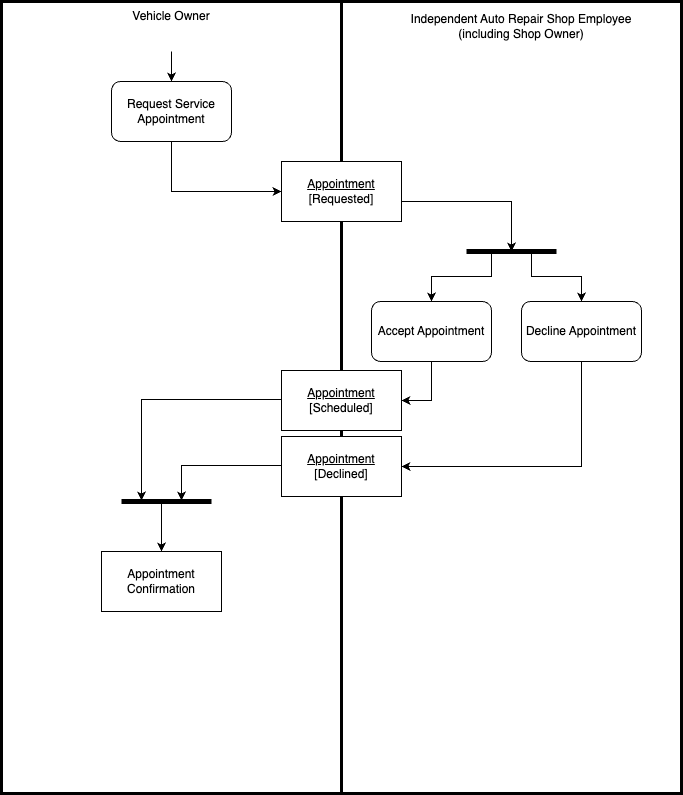
\includegraphics[width=\linewidth/2]{./diagrams/Appointments.png}
	\caption{Service Appointments}
\end{figure}
\FloatBarrier
\begin{figure}[!hbp]
	\centering
	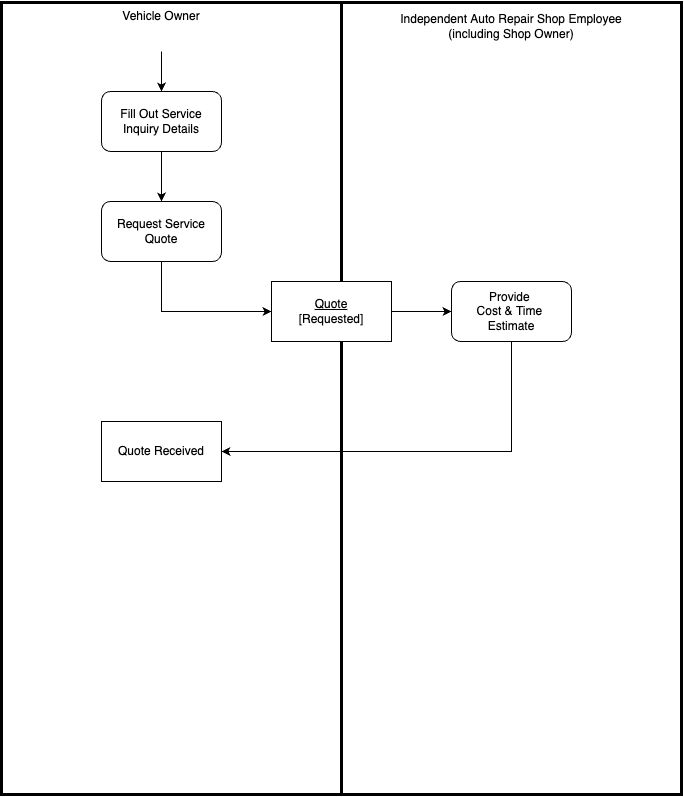
\includegraphics[width=\linewidth/2]{./diagrams/Quotes.png}
	\caption{Service Quotes}
\end{figure}
\FloatBarrier
\begin{figure}[!hbp]
	\centering
	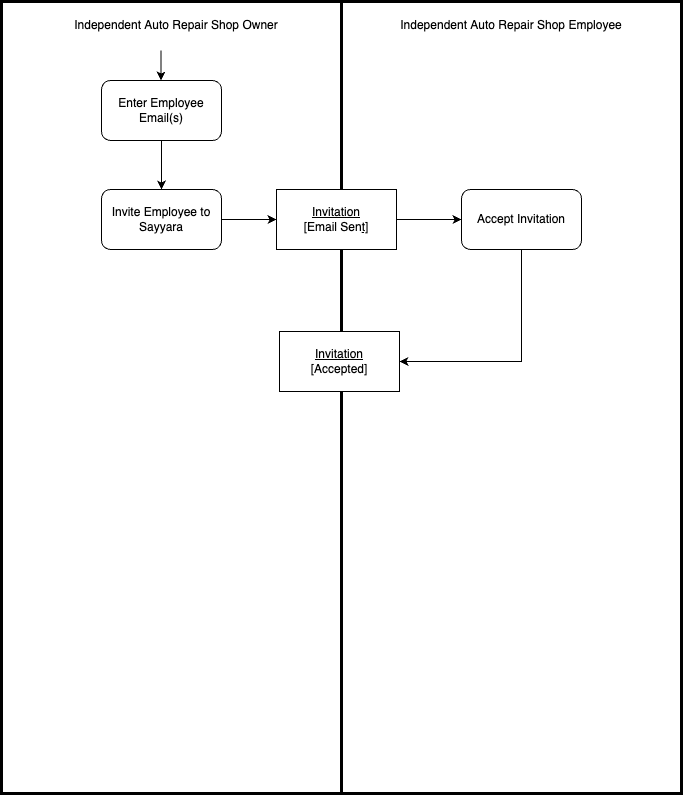
\includegraphics[width=\linewidth/2]{./diagrams/Invitation.png}
	\caption{Employee Invitation to Join Auto Repair Shop}
\end{figure}
\FloatBarrier
\begin{figure}[!hbp]
	\centering
	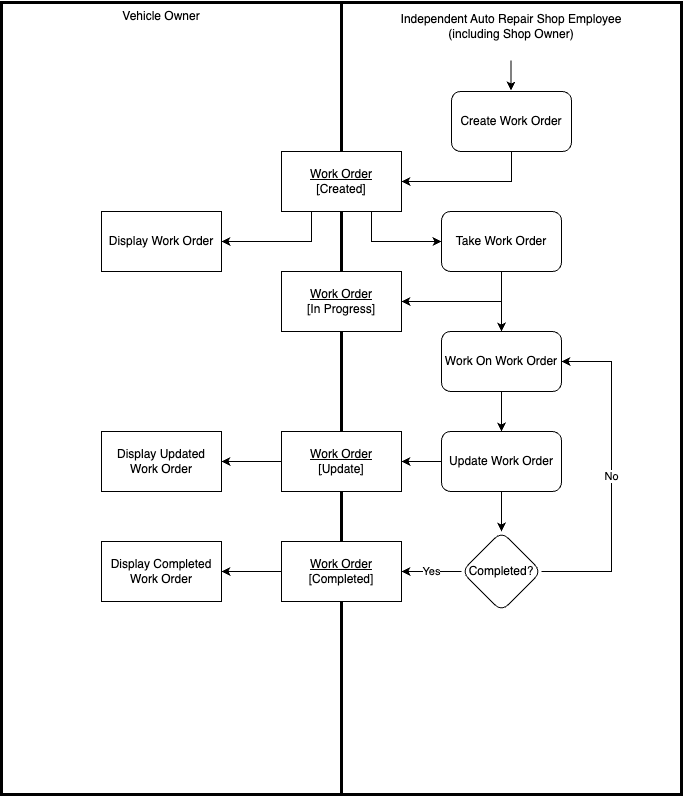
\includegraphics[width=\linewidth/2]{./diagrams/WorkOrder.png}
	\caption{Work Orders}
\end{figure}
\FloatBarrier

\subsubsection{Context of the Work}
The context diagram depicted below illustrates the interactions of the system with adjacent
external systems and services.
\begin{figure}[!hbp]
	\centering
	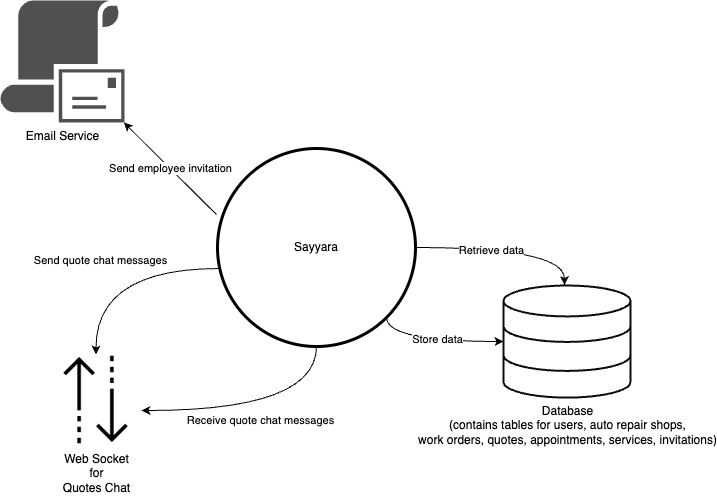
\includegraphics[width=\linewidth/2]{./diagrams/ContextOfWork.png}
	\caption{Context Diagram (Sayyara)}
\end{figure}
\FloatBarrier

\subsubsection{Work Partitioning}

\subsubsection{Individual Product Use Cases}

\subsection{Functional Requirements}
\subsubsection{Authentication}
\begin{enumerate}[label=BE\arabic*., series=business_events]
	\item The user wants to sign up for an account
	      \begin{enumerate}[VP\arabic*.]
		      \item Viewpoint: Vehicle Owner
		            \begin{enumerate}
			            \item The system shall allow the user to enter an email and password
			            \item The system shall allow the user to enter their name
			            \item The system shall allow the user to enter their phone number
			            \item The system shall transition to the vehicle owner landing page after the registration process is
			                  complete and successful
			            \item The system shall allow the user to cancel and exit the registration process
		            \end{enumerate}

		      \item Viewpoint: Auto Repair Shop Owner
		            \begin{enumerate}
			            \item The system shall allow the user to enter an email and password
			            \item The system shall allow the user to enter their name
			            \item The system shall allow the user to enter their phone number
			            \item The system shall allow the user to enter the shop name
			            \item The system shall allow the user to enter the shop address
			            \item The system shall allow the user to enter the shop phone number
			            \item The system shall transition to the shop owner landing page after the registration process is
			                  complete and successful
			            \item The system shall allow the user to cancel and exit the registration process
		            \end{enumerate}

		      \item Viewpoint: Auto Repair Shop Employee
		            \begin{enumerate}
			            \item The system shall allow the user to enter an email and password
			            \item The system shall allow the user to enter their name
			            \item The system shall allow the user to enter their phone number
			            \item The system shall transition to the employee landing page after the registration process is complete
			                  and successful
			            \item The system shall allow the user to cancel and exit the registration process
		            \end{enumerate}
	      \end{enumerate}

	\item The user wants to login to their account
	      \begin{enumerate}[VP\arabic*.]
		      \item Viewpoint: Vehicle Owner
		            \begin{enumerate}
			            \item The system shall allow the user to enter their email and password
			            \item The system shall transition to the vehicle owner landing page after the login process is complete
			                  and successful
			            \item The system shall allow the user to cancel and exit the login process
		            \end{enumerate}

		      \item Viewpoint: Auto Repair Shop Owner
		            \begin{enumerate}
			            \item The system shall allow the user to enter their email and password
			            \item The system shall transition to the shop owner landing page after the login process is complete and
			                  successful
			            \item The system shall allow the user to cancel and exit the login process
		            \end{enumerate}

		      \item Viewpoint: Auto Repair Shop Employee
		            \begin{enumerate}
			            \item The system shall allow the user to enter their email and password
			            \item The system shall transition to the employee landing page after the login process is complete and
			                  successful
			            \item The system shall allow the user to cancel and exit the login process
		            \end{enumerate}
	      \end{enumerate}
\end{enumerate}

\subsubsection{Appointments}
\begin{enumerate}[resume*=business_events]
	\item The user wants to book an appointment
	      \begin{enumerate}[VP\arabic*.]
		      \item Viewpoint: Vehicle Owner
		            \begin{enumerate}
			            \item The system shall populate the service request information from the quote
			            \item The system shall populate the service request information from the if a canned job is selected
			            \item The system shall allow the user to filter available appointments times
			            \item The system shall display dates and times where appointments are available
			            \item The system shall allow the user to select an appointment time slot to book
			            \item The system shall allow the user to sync the appointment time to their calendar
			            \item The system shall transition to the view appointments page
			            \item The system shall allow the user to cancel and exit the appointment process
		            \end{enumerate}
		      \item Viewpoint: Auto Repair Shop Owner
		            \begin{enumerate}
			            \item The system shall allow the user to enter a name
			            \item The system shall allow the user to enter a phone number
			            \item The system shall allow the user to enter service details
			            \item The system shall allow the user to select an available time slot
			            \item The system shall transition to the view appointments page
			            \item The system shall allow the user to cancel and exit the appointment process
		            \end{enumerate}
		      \item Viewpoint: Auto Repair Shop Employee
		            \begin{enumerate}
			            \item The system shall allow the user to enter a name
			            \item The system shall allow the user to enter a phone number
			            \item The system shall allow the user to enter service details
			            \item The system shall allow the user to select an available time slot
			            \item The system shall transition to the view appointments page
			            \item The system shall allow the user to cancel and exit the appointment process
		            \end{enumerate}
	      \end{enumerate}

	\item The user wants to edit an appointment
	      \begin{enumerate}[VP\arabic*.]
		      \item Viewpoint: Vehicle Owner
		            \begin{enumerate}
			            \item The system shall allow the user to select a scheduled appointment
			            \item The system shall allow the user to select another available timeslot
		            \end{enumerate}
		      \item Viewpoint: Auto Repair Shop Owner
		            \begin{enumerate}
			            \item The system shall allow the user to select a scheduled appointment
			            \item The system shall allow the user to update service details
			            \item The system shall allow the user to select another available timeslot
		            \end{enumerate}
		      \item Viewpoint: Auto Repair Shop Employee
		            \begin{enumerate}
			            \item The system shall allow the user to select a scheduled appointment
			            \item The system shall allow the user to update service details
			            \item The system shall allow the user to select another available timeslot
		            \end{enumerate}
	      \end{enumerate}

	\item The user wants to cancel an appointment
	      \begin{enumerate}[VP\arabic*.]
		      \item Viewpoint: Vehicle Owner
		            \begin{enumerate}
			            \item The system shall allow the user to select a scheduled appointment
			            \item The system shall allow the user to cancel the appointment
		            \end{enumerate}
		      \item Viewpoint: Auto Repair Shop Owner
		            \begin{enumerate}
			            \item The system shall allow the user to select a scheduled appointment
			            \item The system shall allow the user to cancel the appointment
		            \end{enumerate}
		      \item Viewpoint: Auto Repair Shop Employee
		            \begin{enumerate}
			            \item The system shall allow the user to select a scheduled appointment
			            \item The system shall allow the user to cancel the appointment
		            \end{enumerate}
	      \end{enumerate}

	\item The user wants to set appointment availability
	      \begin{enumerate}[VP\arabic*.]
		      \item Viewpoint: Vehicle Owner
		            \begin{enumerate}
			            \item[] N/A
		            \end{enumerate}
		      \item Viewpoint: Auto Repair Shop Owner
		            \begin{enumerate}
			            \item The system shall allow the user to set the days that appointments can be made
			            \item The system shall allow the user to set the hours that appointments can be made
			            \item The system shall allow the user to set the number of appointments that can be booked every hour
		            \end{enumerate}
		      \item Viewpoint: Auto Repair Shop Employee
		            \begin{enumerate}
			            \item[] N/A
		            \end{enumerate}
	      \end{enumerate}
\end{enumerate}

\subsubsection{Shop Profile}
\begin{enumerate}[resume*=business_events]
	\item The user wants to view their shop's profile
	      \begin{enumerate}[VP\arabic*.]
		      \item Viewpoint: Auto Repair Shop Owner
		            \begin{enumerate}
			            \item The system shall show the user details of their shop including the shop's location, the shop's
			                  contact information, and a brief description of the shop
		            \end{enumerate}
	      \end{enumerate}
\end{enumerate}

\subsubsection{Employee Profile}
\begin{enumerate}[resume*=business_events]
	\item The user wants to view their employee profile
	      \begin{enumerate}[VP\arabic*.]
		      \item Viewpoint: Auto Repair Shop Employee
		            \begin{enumerate}
			            \item The system shall show the user details of their employee profile, which includes the user's name,
			                  employer details (shop name, employer name), and their position in the auto shop
                \end{enumerate}
        \end{enumerate}
\end{enumerate}

\subsubsection{Work Orders}
\begin{enumerate}[resume*=business_events]
	\item An appointment has been scheduled
	      \begin{enumerate}[VP\arabic*.]
		      \item Viewpoint: Vehicle Owner
		            \begin{enumerate}
			            \item[] N/A
		            \end{enumerate}
		      \item Viewpoint: Auto Repair Shop Owner
		            \begin{enumerate}
			            \item The system shall create a work order
			            \item The system shall populate the customer data and vehicle data from the quote
			            \item The system shall populate the customer data and vehicle data from the appointment if the quote is
			                  not available
			            \item The system shall populate expected services performed and parts needed from the quote
			            \item The system shall populate expected services performed and parts needed from the appointment if the
			                  quote not available
		            \end{enumerate}
		      \item Viewpoint: Auto Repair Shop Employee
		            \begin{enumerate}
			            \item The system shall create a work order
			            \item The system shall populate the customer data and vehicle data from the quote
			            \item The system shall populate the customer data and vehicle data from the appointment if the quote is
			                  not available
			            \item The system shall populate expected services performed and parts needed from the quote
			            \item The system shall populate expected services performed and parts needed from the appointment if the
			                  quote not available
		            \end{enumerate}
	      \end{enumerate}

	\item An appointment has been cancelled
	      \begin{enumerate}[VP\arabic*.]
		      \item Viewpoint: Vehicle Owner
		            \begin{enumerate}
			            \item[] N/A
		            \end{enumerate}
		      \item Viewpoint: Auto Repair Shop Owner
		            \begin{enumerate}
			            \item The system shall delete the associated work order
		            \end{enumerate}
		      \item Viewpoint: Auto Repair Shop Employee
		            \begin{enumerate}
			            \item The system shall delete the associated work order
		            \end{enumerate}
	      \end{enumerate}

	\item The user wants to search for a work order
	      \begin{enumerate}[VP\arabic*.]
		      \item Viewpoint: Vehicle Owner
		            \begin{enumerate}
			            \item[] N/A
		            \end{enumerate}
		      \item Viewpoint: Auto Repair Shop Owner
		            \begin{enumerate}
			            \item The system shall allow the user to enter the customer name, assigned employee, service type, and a
			                  date range
			            \item The system shall list the work order matching the inputted criteria
		            \end{enumerate}
		      \item Viewpoint: Auto Repair Shop Employee
		            \begin{enumerate}
			            \item The system shall allow the user to enter the customer name, assigned employee, service type, and a
			                  date range
			            \item The system shall list the work order matching the inputted criteria
		            \end{enumerate}
	      \end{enumerate}

	\item The user wants to view past work orders
	      \begin{enumerate}[VP\arabic*.]
		      \item Viewpoint: Vehicle Owner
		            \begin{enumerate}
			            \item[] N/A
		            \end{enumerate}
		      \item Viewpoint: Auto Repair Shop Owner
		            \begin{enumerate}
			            \item The system shall list the past work orders
		            \end{enumerate}
		      \item Viewpoint: Auto Repair Shop Employee
		            \begin{enumerate}
			            \item The system shall list the past work orders
		            \end{enumerate}
	      \end{enumerate}

	\item The user wants update an work order
	      \begin{enumerate}[VP\arabic*.]
		      \item Viewpoint: Vehicle Owner
		            \begin{enumerate}
			            \item[] N/A
		            \end{enumerate}
		      \item Viewpoint: Auto Repair Shop Owner
		            \begin{enumerate}
			            \item The system shall list the open work orders
			            \item The system shall allow the user to edit the services performed, parts required, odometer readings,
			                  customer details, employee assigned, car details, discounts, digital vehicle inspection, and extra
			                  notes
			            \item The system shall update the work order with the entered values
		            \end{enumerate}
		      \item Viewpoint: Auto Repair Shop Employee
		            \begin{enumerate}
			            \item The system shall list the open work orders
			            \item The system shall allow the user to edit the services performed, parts required, odometer readings,
			                  customer details, employee assigned, car details, discounts, digital vehicle inspection, and extra
			                  notes
			            \item The system shall update the work order with the entered values
		            \end{enumerate}
	      \end{enumerate}

	\item The customer has paid for the work done on their vehicle
	      \begin{enumerate}[VP\arabic*.]
		      \item Viewpoint: Vehicle Owner
		            \begin{enumerate}
			            \item[] N/A
		            \end{enumerate}
		      \item Viewpoint: Auto Repair Shop Owner
		            \begin{enumerate}
			            \item The system shall send a copy of the work order to the assigned customer's email
			            \item The system shall mark the work order as ``Completed''
			            \item The system shall mark the associated appointment as ``Completed''
		            \end{enumerate}
		      \item Viewpoint: Auto Repair Shop Employee
		            \begin{enumerate}
			            \item The system shall send a copy of the work order to the assigned customer's email
			            \item The system shall mark the work order as ``Completed''
			            \item The system shall mark the associated appointment as ``Completed''
		            \end{enumerate}
	      \end{enumerate}

	\item The user wants to view the details of a work order
	      \begin{enumerate}[VP\arabic*.]
		      \item Viewpoint: Vehicle Owner
		            \begin{enumerate}
			            \item[] N/A
		            \end{enumerate}
		      \item Viewpoint: Auto Repair Shop Owner
		            \begin{enumerate}
			            \item The system shall list the shop details, services to be performed with their individual bill rates
			                  and expected number of hours for completion, parts required and their cost, odometer reading before
			                  and after service, customer details, assigned employee, car details, any applied discounts, final
			                  balance for the customer, warranty information, digital vehicle inspection, and any extra notes
		            \end{enumerate}
		      \item Viewpoint: Auto Repair Shop Employee
		            \begin{enumerate}
			            \item The system shall list the shop details, services to be performed with their individual bill rates
			                  and expected number of hours for completion, parts required and their cost, odometer reading before
			                  and after service, customer details, assigned employee, car details, any applied discounts, final
			                  balance for the customer, warranty information, digital vehicle inspection, and any extra notes
		            \end{enumerate}
	      \end{enumerate}

\end{enumerate}

\subsubsection{Employee Management}
\begin{enumerate}[resume*=business_events]
	\item The shop owner wants to invite an employee to their shop
	      \begin{enumerate}[VP\arabic*.]
		      \item Viewpoint: Vehicle Owner
		            \begin{enumerate}
			            \item[] N/A
		            \end{enumerate}
		      \item Viewpoint: Auto Repair Shop Owner
		            \begin{enumerate}
			            \item The system shall allow the user to enter employee email(s) to invite
			            \item The system shall send an invitation email to the invited employee(s)
		            \end{enumerate}
		      \item Viewpoint: Auto Repair Shop Employee
		            \begin{enumerate}
			            \item The system shall allow the user to accept an invitation
		            \end{enumerate}
	      \end{enumerate}

	\item The shop owner wants to search for an employee
	      \begin{enumerate}[VP\arabic*.]
		      \item Viewpoint: Vehicle Owner
		            \begin{enumerate}
			            \item[] N/A
		            \end{enumerate}
		      \item Viewpoint: Auto Repair Shop Owner
		            \begin{enumerate}
			            \item The system shall allow the user to enter search text to search for an employee
			            \item The system shall display a list of employees whose name or email matches the search text
		            \end{enumerate}
		      \item Viewpoint: Auto Repair Shop Employee
		            \begin{enumerate}
			            \item[] N/A
		            \end{enumerate}
	      \end{enumerate}

	\item The shop owner wants to view the list of employees
	      \begin{enumerate}[VP\arabic*.]
		      \item Viewpoint: Vehicle Owner
		            \begin{enumerate}
			            \item[] N/A
		            \end{enumerate}
		      \item Viewpoint: Auto Repair Shop Owner
		            \begin{enumerate}
			            \item The system shall display a list of employees
		            \end{enumerate}
		      \item Viewpoint: Auto Repair Shop Employee
		            \begin{enumerate}
			            \item[] N/A
		            \end{enumerate}
	      \end{enumerate}

	\item The shop owner wants to remove an employee
	      \begin{enumerate}[VP\arabic*.]
		      \item Viewpoint: Vehicle Owner
		            \begin{enumerate}
			            \item[] N/A
		            \end{enumerate}
		      \item Viewpoint: Auto Repair Shop Owner
		            \begin{enumerate}
			            \item The system shall allow the user to remove an employee
			            \item The system shall revoke the removed employee's access to the auto repair shop employee controls
		            \end{enumerate}
		      \item Viewpoint: Auto Repair Shop Employee
		            \begin{enumerate}
			            \item The system shall revoke the removed employee's access to the auto repair shop employee controls
		            \end{enumerate}
	      \end{enumerate}
\end{enumerate}

\subsubsection{Services}
\begin{enumerate}[resume*=business_events]
	\item The user wants to add available auto shop services to the shop profile
	      \begin{enumerate}[VP\arabic*.]
		      \item Viewpoint: Vehicle Owner
		            \begin{enumerate}
			            \item[] N/A
		            \end{enumerate}
		      \item Viewpoint: Auto Repair Shop Owner
		            \begin{enumerate}
			            \item The system shall allow the user to enter the name of the service
			            \item The system shall allow the user to enter a description for the service
			            \item The system shall allow the user to enter the estimated time for the service
			            \item The system shall allow the user to enter the parts used for the service including quantity,
			                  condition (new or used), build (OEM or aftermarket), and cost per part (before tax cost)
			            \item The system shall allow the user to enter the total price for the service (before tax price)
		            \end{enumerate}
		      \item Viewpoint: Auto Repair Shop Employee
		            \begin{enumerate}
			            \item[] N/A
		            \end{enumerate}
	      \end{enumerate}

	\item The user wants to search for auto repair or maintenance services
	      \begin{enumerate}[VP\arabic*.]
		      \item Viewpoint: Vehicle Owner
		            \begin{enumerate}
			            \item The system shall display the service details
		            \end{enumerate}
		      \item Viewpoint: Auto Repair Shop Owner
		            \begin{enumerate}
			            \item The system shall display the service details
			            \item The system shall allow the user to search for a specific service type
		            \end{enumerate}
		      \item Viewpoint: Auto Repair Shop Employee
		            \begin{enumerate}
			            \item The system shall display the service details
			            \item The system shall allow the user to search for a specific service type
		            \end{enumerate}
	      \end{enumerate}

	\item The user wants to edit a service type
	      \begin{enumerate}[VP\arabic*.]
		      \item Viewpoint: Vehicle Owner
		            \begin{enumerate}
			            \item[] N/A
		            \end{enumerate}
		      \item Viewpoint: Auto Repair Shop Owner
		            \begin{enumerate}
			            \item The system shall allow the user to update the details of a particular service
		            \end{enumerate}
		      \item Viewpoint: Auto Repair Shop Employee
		            \begin{enumerate}
			            \item[] N/A
		            \end{enumerate}
	      \end{enumerate}

	\item The user wants to delete a service type
	      \begin{enumerate}[VP\arabic*.]
		      \item Viewpoint: Vehicle Owner
		            \begin{enumerate}
			            \item[] N/A
		            \end{enumerate}
		      \item Viewpoint: Auto Repair Shop Owner
		            \begin{enumerate}
			            \item The system shall allow the user to delete the service from their shop page
		            \end{enumerate}
		      \item Viewpoint: Auto Repair Shop Employee
		            \begin{enumerate}
			            \item[] N/A
		            \end{enumerate}
	      \end{enumerate}
\end{enumerate}

\section{Non-functional Requirements}

\subsection{Look and Feel Requirements}

\subsection{Usability and Humanity Requirements}

\subsection{Performance Requirements}

\subsection{Operational and Environmental Requirements}

\subsection{Maintainability and Support Requirements}

\subsection{Security Requirements}

\subsection{Cultural Requirements}

\subsection{Legal Requirements}

\subsection{Health and Safety Requirements}

This section is not in the original Volere template, but health and safety are issues that should
be considered for every engineering project.

\section{Project Issues}

\subsection{Open Issues}

\subsection{Off-the-Shelf Solutions}

\subsection{New Problems}

\subsection{Tasks}

\subsection{Migration to the New Product}

\subsection{Risks}

\subsection{Costs}

\subsection{User Documentation and Training}

\subsection{Waiting Room}

\subsection{Ideas for Solutions}

\newpage

\bibliographystyle{plainnat}

\bibliography {../../refs/References}

\newpage

\noindent \plt{The following is not part of the template, just some things to consider
	when filing in the template.}

\noindent \plt{Grammar, flow and \LaTeX advice:
	\begin{itemize}
		\item For Mac users \texttt{*.DS\_Store} should be in \texttt{.gitignore}
		\item \LaTeX{} and formatting rules
		      \begin{itemize}
			      \item Variables are italic, everything else not, includes subscripts (link to document)
			            \begin{itemize}
				            \item \href{https://physics.nist.gov/cuu/pdf/typefaces.pdf}{Conventions}
				            \item Watch out for implied multiplication
			            \end{itemize}
			      \item Use BibTeX
			      \item Use cross-referencing
		      \end{itemize}
		\item Grammar and writing rules
		      \begin{itemize}
			      \item Acronyms expanded on first usage (not just in table of acronyms)
			      \item ``In order to'' should be ``to''
		      \end{itemize}
	\end{itemize}}

\noindent \plt{Advice on using the template:
	\begin{itemize}
		\item Difference between physical and software constraints
		\item Properties of a correct solution means \emph{additional} properties, not a restating of the
		      requirements (may be ``not applicable'' for your problem). If you have a table of output
		      constraints, then these are properties of a correct solution.
		\item Assumptions have to be invoked somewhere
		\item ``Referenced by'' implies that there is an explicit reference
		\item Think of traceability matrix, list of assumption invocations and list of reference by fields as
		      automatically generatable
		\item If you say the format of the output (plot, table etc), then your requirement could be more abstract
	\end{itemize}
}
\section{Appendix}

This section has been added to the Volere template. This is where you can place additional
information.

\newpage{}
\subsection{Reflection}

The information in this section will be used to evaluate the team members on the graduate attribute
of Lifelong Learning. Please answer the following questions:

\begin{enumerate}
	\item What knowledge and skills will the team collectively need to acquire to successfully complete this
	      capstone project? Examples of possible knowledge to acquire include domain specific knowledge from
	      the domain of your application, or software engineering knowledge, mechatronics knowledge or
	      computer science knowledge. Skills may be related to technology, or writing, or presentation, or
	      team management, etc. You should look to identify at least one item for each team member.
	\item For each of the knowledge areas and skills identified in the previous question, what are at least
	      two approaches to acquiring the knowledge or mastering the skill? Of the identified approaches,
	      which will each team member pursue, and why did they make this choice?
\end{enumerate}

\subsection{Symbolic Parameters}

The definition of the requirements will likely call for SYMBOLIC\_CONSTANTS. Their values are
defined in this section for easy maintenance.

\end{document}